\documentclass{article}
%\usepackage[margin=1in]{geometry}
\usepackage{graphicx} % Required for inserting images
\usepackage{hyperref}
\usepackage{amsmath}
\usepackage{titling}
\usepackage{enumitem}
\usepackage{makecell}
\usepackage{minted}
\usepackage{url}
\usepackage{tabularx}
\usepackage{graphicx}
\renewcommand\maketitlehooka{\null\mbox{}\vfill}
\renewcommand\maketitlehookd{\vfill\null}

\begin{document}
\centering

\title{\Huge Intro Deep Learning Homework 1}

\author{ \huge
Jaskin Kabir \\
\Large Student Id: 801186717 \\
\Large \href{https://github.com/jaskinkabir/Intro_Deep_Learning/tree/master/HM1}{GitHub:}\\\url{https://github.com/jaskinkabir/Intro_Deep_Learning/tree/master/HM1}
}

\date{January 2025}

\begin{titlingpage}
\maketitle
\end{titlingpage}

\section{Problem 1: Character Prediction Small Dataset}

\begin{enumerate}[label=1\alph*. ]
    \item waaa
    \begin{figure}[htb]
        \setkeys{Gin}{width=\linewidth}
        \setlength\tabcolsep{2pt}
        \begin{tabularx}{\textwidth}{XXX}
          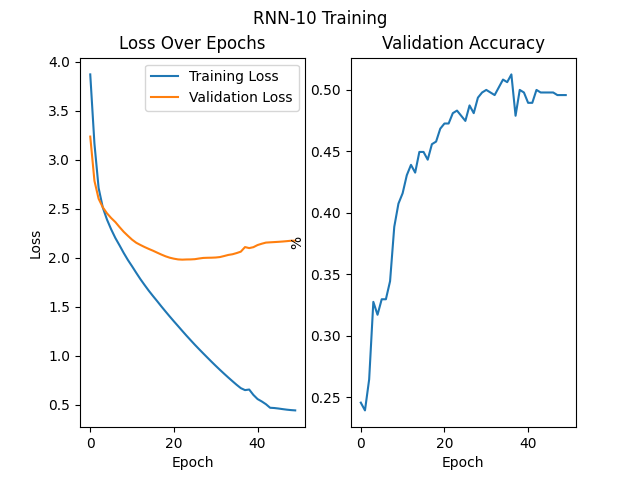
\includegraphics{images_p1/RNN_10_training_new.png} &
          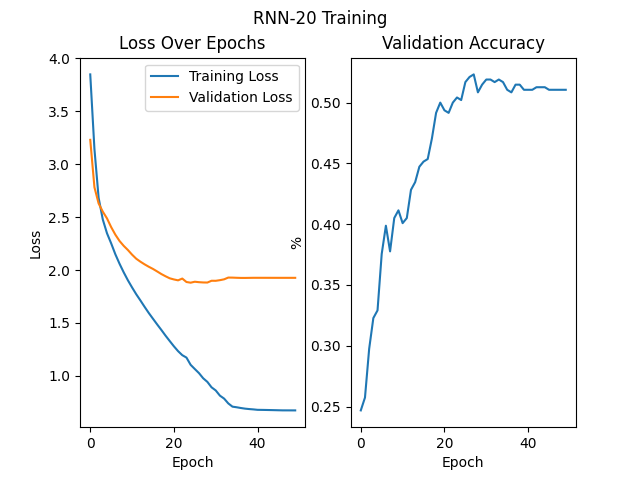
\includegraphics{images_p1/RNN_20_training_new.png} &
          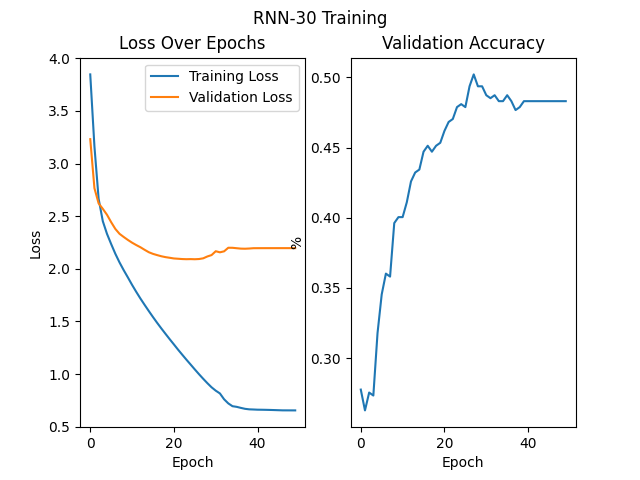
\includegraphics{images_p1/RNN_30_training_new.png}   \\
          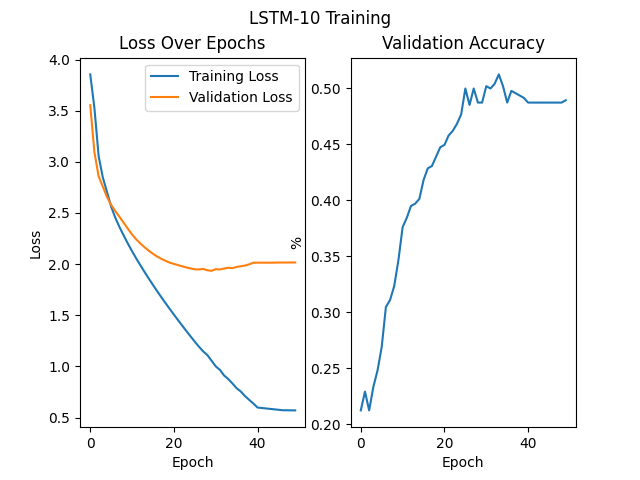
\includegraphics{images_p1/LSTM_10_training_new.png} &
          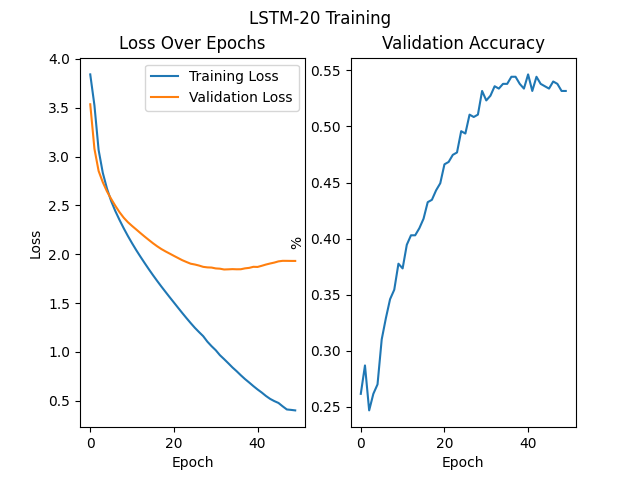
\includegraphics{images_p1/LSTM_20_training_new.png} &
          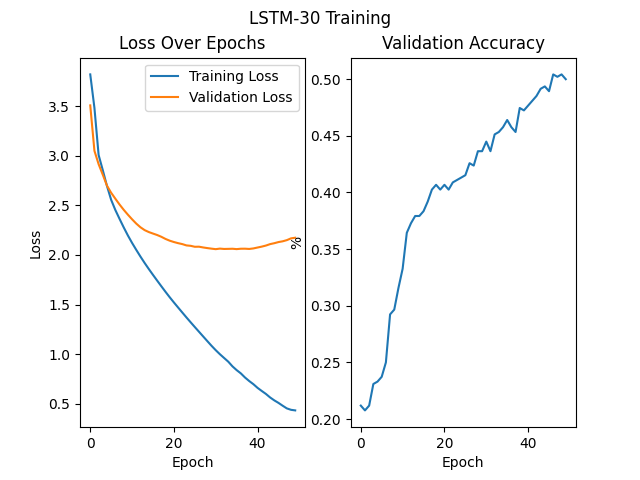
\includegraphics{images_p1/LSTM_30_training_new.png}   \\
          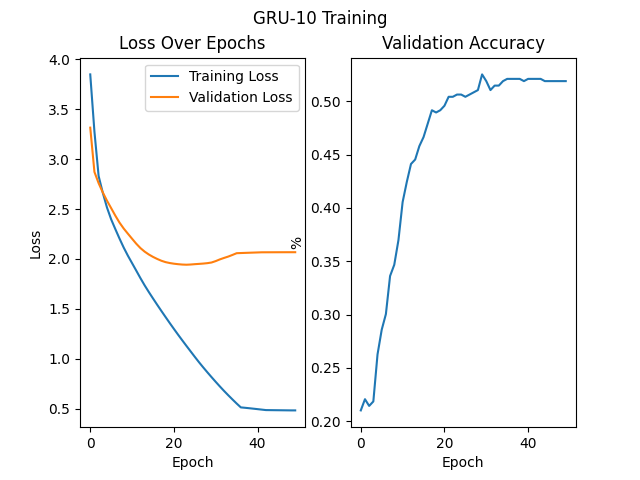
\includegraphics{images_p1/GRU_10_training_new.png} &
          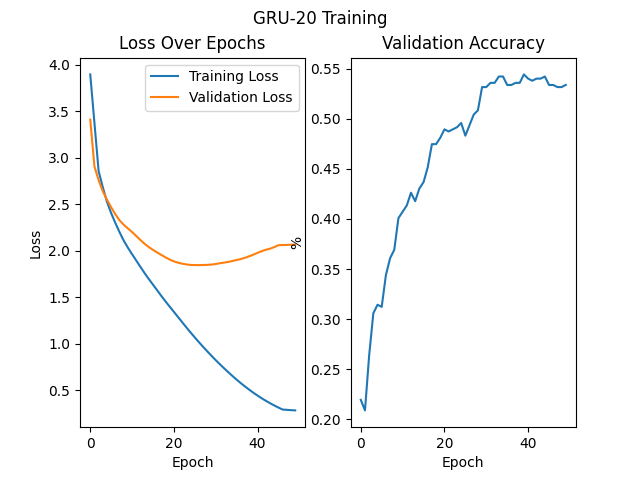
\includegraphics{images_p1/GRU_20_training_new.png} &
          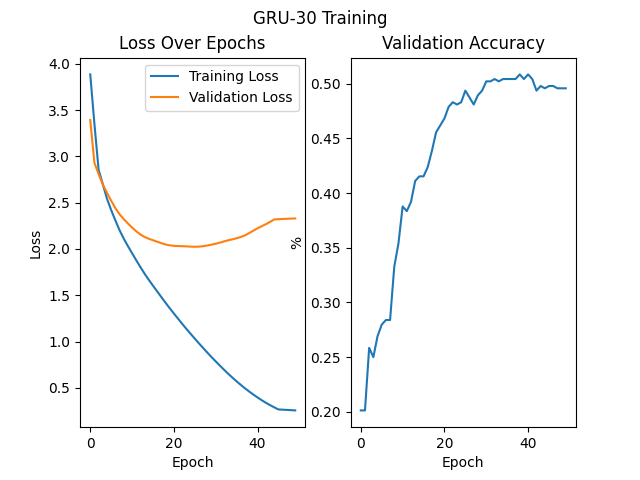
\includegraphics{images_p1/GRU_30_training_new.png}
        \end{tabularx}
      \caption{Set graphics options by keys "Gin"}
      \end{figure}
\end{enumerate}


\end{document}